\chapter{Introduction}
\label{ch:intro}

\section{Background}
\label{sect:background}

In the early 1990's, there was a lack of quantitative studies on the characterization of a side-dump combustor's flow field. These types of combustors are generally found in solid-propellant ducted rocket ramjets. In Figure~\ref{fig:config} below, the configuration for such a combustor is shown.

\begin{figure}[H]
	\centering
	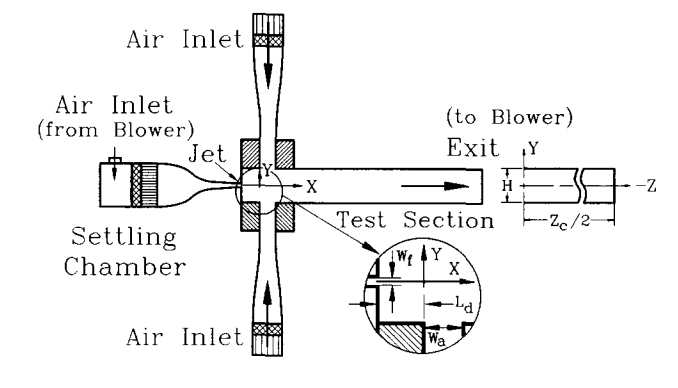
\includegraphics[scale=0.4]{ref/config}
	\caption[Side-dump combustor's experimental configuration.]{Side dump combustor's experimental configuration. \cite{art}}
	\label{fig:config}
\end{figure}

This was the motivation for \cite{art}, who characterized the flow field using laser-Doppler velocimetry techniques. Mean velocities, turbulent kinetic energy and Reynolds stresses were measured. This study serves as a background for this report.

\section{Purpose}
\label{sect:purpose}

The purpose of this report is to determine the effects of side inlet angle on the combustor's mixing capabilities \cite{proj} using \cite{cfx}. Specifically, counter-clockwise (CCW) and clockwise (CW) angles of -20\textsuperscript{o} and 10\textsuperscript{o}, respectively, are of interest. 


\section{Scope}
In this report, the CFX-Prev environment for all three models is presented. Results for each simulation are then discussed and compared with experimental results from \cite{art}. Based on findings, respective conclusions on the effect of side inlet angle are made. Mixing will be quantified in using temperature as a passive fluid marker \cite{proj}.
